\documentclass[a4paper, 12pt]{report}

%====================== PACKAGES ======================

\usepackage[french]{babel}
\usepackage[utf8x]{inputenc}
%pour gérer les positionnement d'images
\usepackage{float}
\usepackage{amsmath}
\usepackage{graphicx}
\usepackage[colorinlistoftodos]{todonotes}
\usepackage{url}
%pour les informations sur un document compilé en PDF et les liens externes / internes
\usepackage{hyperref}
%pour la mise en page des tableaux
\usepackage{array}
\usepackage{tabularx}
%pour utiliser \floatbarrier
%\usepackage{placeins}
%\usepackage{floatrow}
%espacement entre les lignes
\usepackage{setspace}
%modifier la mise en page de l'abstract
\usepackage{abstract}
%police et mise en page (marges) du document
\usepackage[T1]{fontenc}
\usepackage[top=2cm, bottom=2cm, left=2cm, right=2cm]{geometry}
%Pour les galerie d'images
\usepackage{subfig}

%====================== INFORMATION ET REGLES ======================

%rajouter les numérotation pour les \paragraphe et \subparagraphe
\setcounter{secnumdepth}{4}
\setcounter{tocdepth}{4}

\hypersetup{							% Information sur le document
pdfauthor = {Sugdenaz EKICI,
			Yahia KHERZA,
			Olivier MARAVAL,
    		Valentin VIRET-JACQUOT},			% Auteurs
pdftitle = {1_Analyse},			% Titre du document
pdfsubject = {Mémoire de Projet},		% Sujet
pdfkeywords = {Tag1, Tag2, Tag3, ...},	% Mots-clefs
pdfstartview={FitH}}					% ajuste la page à la largueur de l'écran
%pdfcreator = {MikTeX},% Logiciel qui a crée le document
%pdfproducer = {}} % Société avec produit le logiciel

%======================== DEBUT DU DOCUMENT ========================

\begin{document}

\addtocontents{toc}{\protect\thispagestyle{empty}}

%régler l'espacement entre les lignes
\newcommand{\HRule}{\rule{\linewidth}{0.5mm}}

%page de garde
\begin{titlepage}
\begin{center}

% Upper part of the page. The '~' is needed because only works if a paragraph has started.

\includegraphics[width=0.5\textwidth]{./images/InfoLogoQuadriH.png}~\\[1cm]

\textsc{\LARGE SAE 1.04 - BUT INFORMATIQUE - GROUPE 1}\\[1.5cm]

\textsc{\Large }\\[0.5cm]

% Title
\HRule \\[0.4cm]

{\huge \bfseries Analyse des besoins de l'entreprise\\
 LOCECO\\[0.4cm] }

\HRule \\[1.5cm]

% Author and supervisor
\begin{minipage}{0.4\textwidth}
\begin{flushleft} \large
\emph{Auteur:}\\
Sugdenaz \textsc{Ekici}(\textit{A1})\\
Yahia \textsc{Kherza}(\textit{A1})\\
Olivier \textsc{Maraval}(\textit{A1})\\
Valentin \textsc{Viret-Jacquot}(\textit{A1})
\end{flushleft}
\end{minipage}
\begin{minipage}{0.4\textwidth}
\begin{flushright} \large
\emph{Client:} \\
Karine \textsc{Deschinkel}\\
\emph{Référent:} \\
Olivier \textsc{Maraval}
\end{flushright}
\end{minipage}

\vfill

% Bottom of the page
{\large \today}

\end{center}
\end{titlepage}

%page blanche
\newpage
~
%ne pas numéroter cette page
\thispagestyle{empty}
\newpage

\renewcommand{\abstractnamefont}{\normalfont\Large\bfseries}
%\renewcommand{\abstracttextfont}{\normalfont\Huge}

\begin{abstract}
\hskip7mm

\begin{spacing}{1.3}

Lorem ipsum dolor sit amet, consectetur adipiscing elit. Sed non risus. Suspendisse lectus tortor, dignissim sit amet, adipiscing nec, ultricies sed, dolor. Cras elementum ultrices diam. Maecenas ligula massa, varius a, semper congue, euismod non, mi. Proin porttitor, orci nec nonummy molestie, enim est eleifend mi, non fermentum diam nisl sit amet erat. Duis semper. Duis arcu massa, scelerisque vitae, consequat in, pretium a, enim. Pellentesque congue. Ut in risus volutpat libero pharetra tempor. Cras vestibulum bibendum augue. Praesent egestas leo in pede. Praesent blandit odio eu enim. Pellentesque sed dui ut augue blandit sodales. Vestibulum ante ipsum primis in faucibus orci luctus et ultrices posuere cubilia Curae; Aliquam nibh. Mauris ac mauris sed pede pellentesque fermentum. Maecenas adipiscing ante non diam sodales hendrerit. Ut velit mauris, egestas sed, gravida nec, ornare ut, mi. Aenean ut orci vel massa suscipit pulvinar. Nulla sollicitudin. Fusce varius, ligula non tempus aliquam, nunc turpis ullamcorper nibh, in tempus sapien eros vitae ligula. Pellentesque rhoncus nunc et augue. Integer id felis. Curabitur aliquet pellentesque diam. Integer quis metus vitae elit lobortis egestas. Lorem ipsum dolor sit amet, consectetuer adipiscing elit. Morbi vel erat non mauris convallis vehicula. Nulla et sapien. Integer tortor tellus, aliquam faucibus, convallis id, congue eu, quam. Mauris ullamcorper felis vitae erat. Proin feugiat, augue non elementum posuere, metus purus iaculis lectus, et tristique ligula justo vitae magna. Aliquam convallis sollicitudin purus. Praesent aliquam, enim at fermentum mollis, ligula massa adipiscing nisl, ac euismod nibh nisl eu lectus. Fusce vulputate sem at sapien. Vivamus leo. Aliquam euismod libero eu enim. Nulla nec felis sed leo placerat imperdiet. Aenean suscipit nulla in justo. Suspendisse cursus rutrum augue. Nulla tincidunt tincidunt mi. Curabitur iaculis, lorem vel rhoncus faucibus, felis magna fermentum augue, et ultricies lacus lorem varius purus. Curabitur eu amet.

\end{spacing}
\end{abstract}



\tableofcontents
\thispagestyle{empty}

%ne pas numéroter le sommaire

\newpage

%espacement entre les lignes d'un tableau
\renewcommand{\arraystretch}{1.5}

%====================== INCLUSION DES PARTIES ======================

~
\thispagestyle{empty}


\newpage
%recommencer la numérotation des pages à "7"
\setcounter{page}{7}

\chapter{Analyse de l'existant}

\section{Les écoquartiers}

\subsection{Présentation du concept d'écoquartier}

Un écoquartier est un quartier urbain conçu de manière à être respectueux de l'environnement et à promouvoir le développement durable. Il intègre des principes tels que la gestion efficace des ressources, la réduction des émissions de carbone, la promotion de la mobilité douce et l'utilisation d'énergies renouvelables.\\

Le fonctionnement d'un écoquartier repose sur plusieurs principes clés :
\begin{itemize}
\item \textbf{La gestion efficace des ressources :} un écoquartier vise à minimiser la consommation d'eau et d'énergie, ainsi que la production de déchets. Cela peut se faire en utilisant des technologies d'énergie renouvelable, en encourageant la réutilisation et le recyclage des matériaux, ou encore en favorisant les modes de transport doux comme le vélo ou les transports en commun.
\item \textbf{La conception urbaine durable :} un écoquartier est conçu pour encourager la cohésion sociale, en offrant des espaces verts et des lieux de rencontre pour les résidents. Il doit également être accessible à tous, notamment aux personnes à mobilité réduite.
\item \textbf{La participation des résidents :} les habitants de l'écoquartier sont encouragés à participer activement à la gestion du quartier, en prenant part aux décisions concernant l'aménagement et l'utilisation des espaces communs.
\item \textbf{La promotion de l'économie locale :} un écoquartier peut encourager l'installation d'entreprises locales et durables, favorisant ainsi l'emploi et l'économie locale.
\end{itemize}


\subsection{Exemple d'écoquartier}

Le quartier Vauban à Fribourg-en-Brisgau, en Allemagne est un exemple d'écoquartier. Ce dernier est conçu de manière à encourager la marche à pied et le vélo, avec des rues piétonnes et des pistes cyclables bien développées. 

Il utilise également des technologies d'énergie renouvelable, telles que l'énergie solaire, pour alimenter les bâtiments. De plus, le quartier favorise la cohésion sociale en encourageant la participation des résidents à la gestion du quartier et en offrant des espaces verts et des jardins communautaires.

\begin{figure}[!h]
\begin{center}
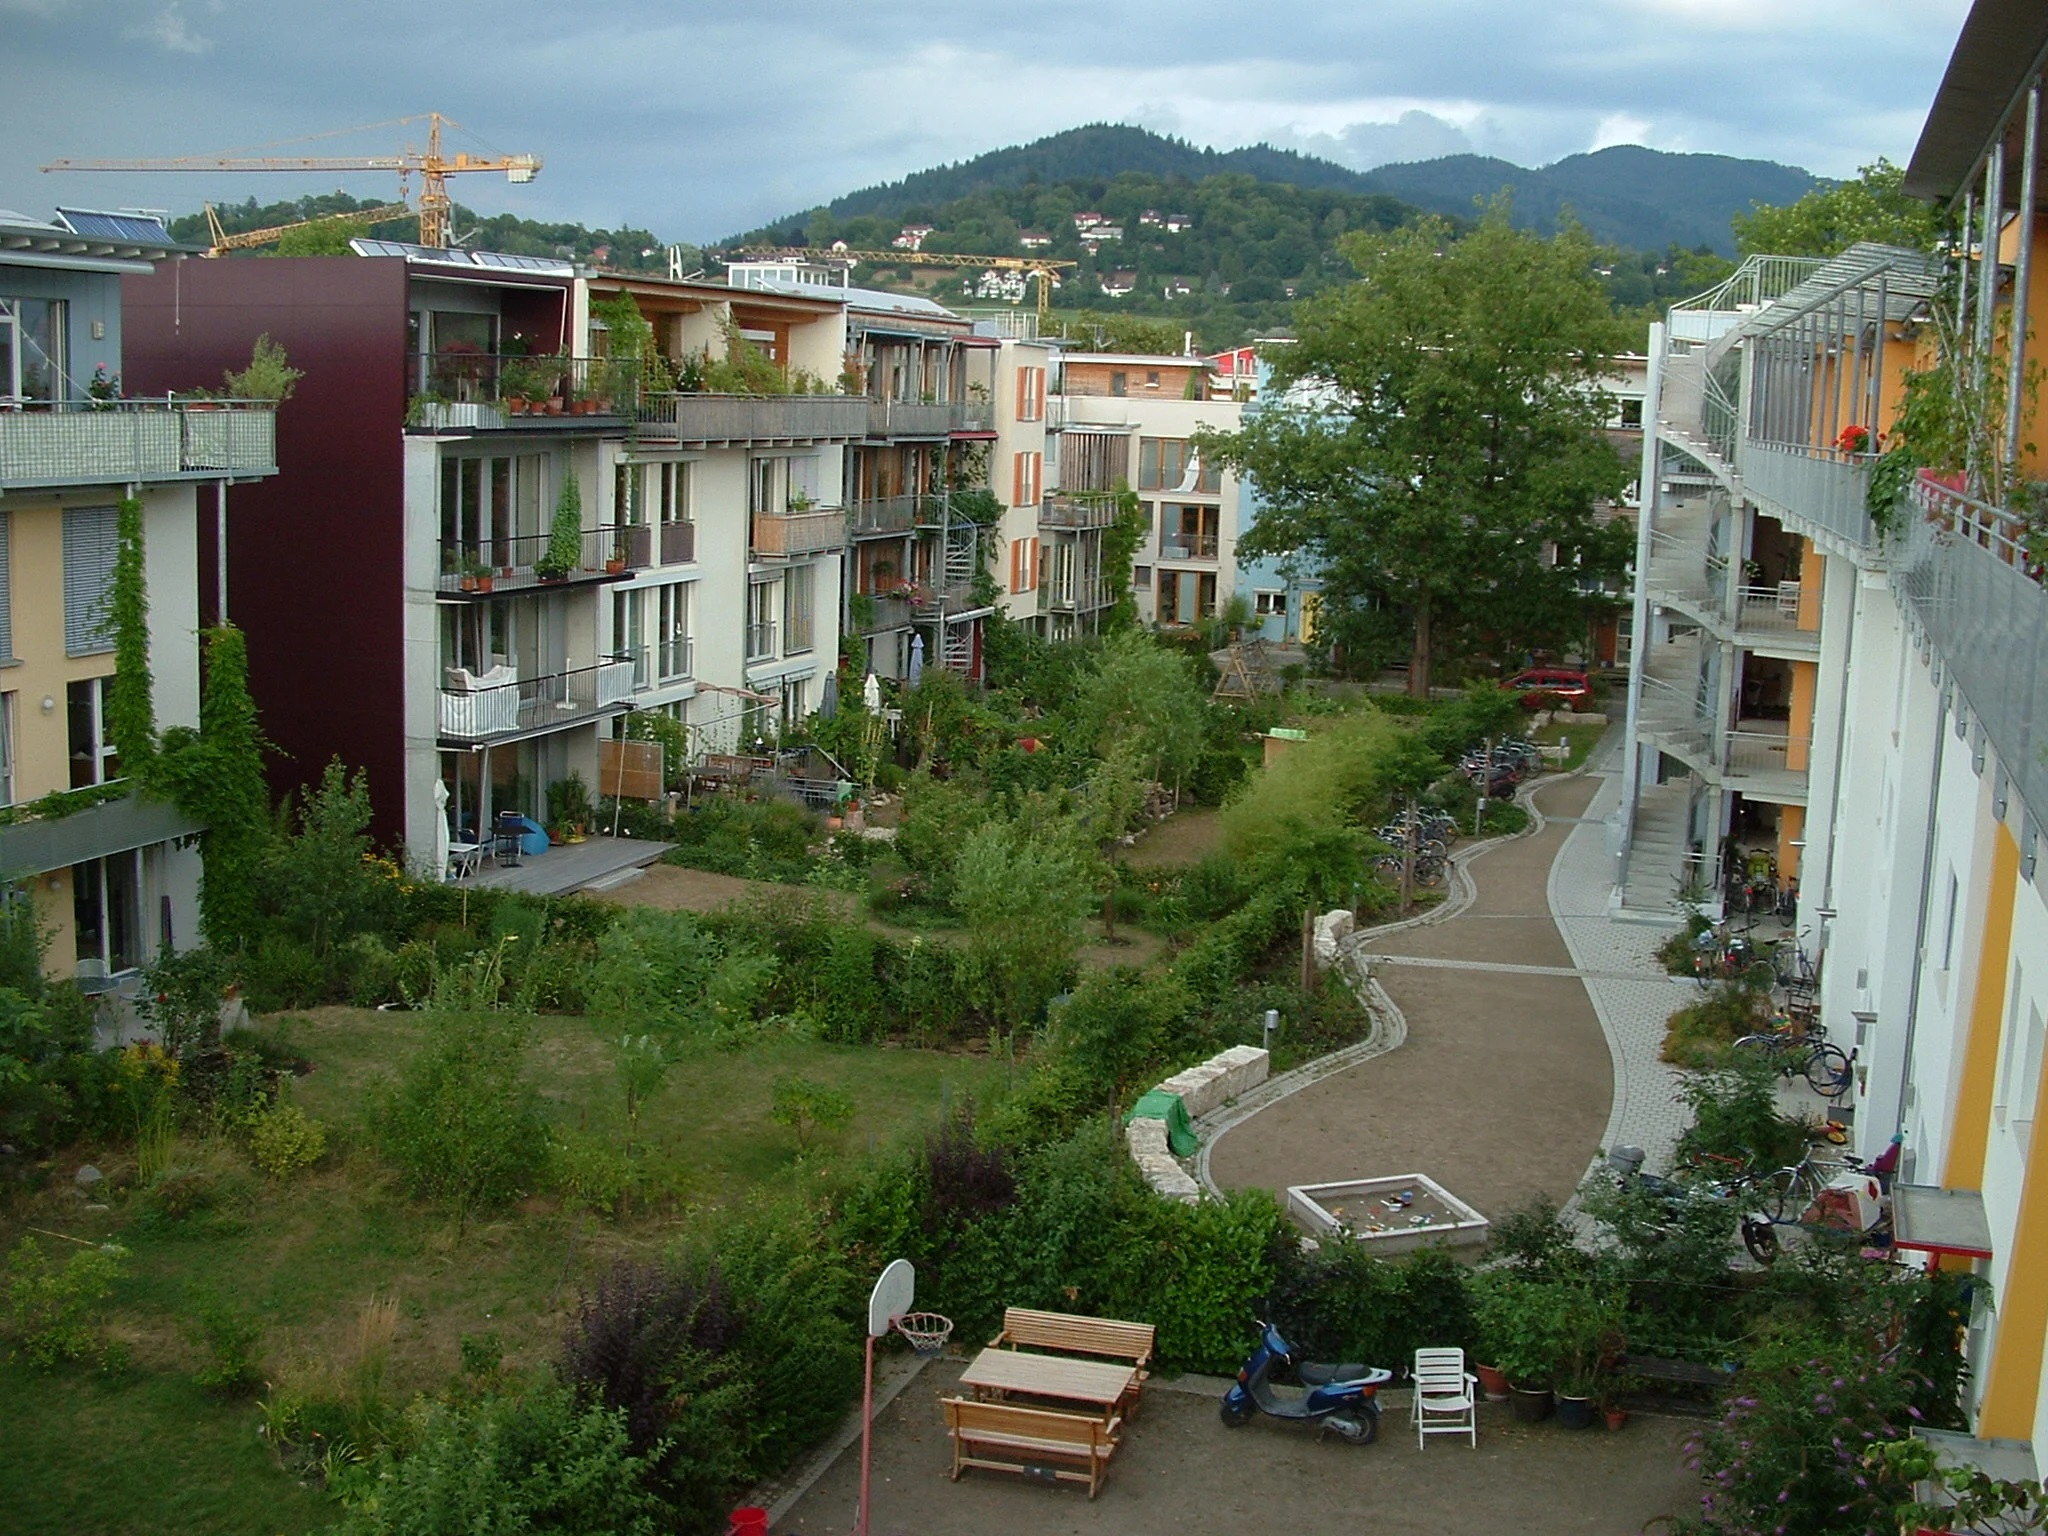
\includegraphics[width=15cm]{vauban-10029.jpg}
\end{center}
\caption{Le quartier Vauban à Fribourg-en-Brisgau}
\end{figure}

\newpage

\section{L'entreprise et l'écoquartier}

\subsection{Présentation de LOCECO}

LOCECO est une entreprise engagée dans la gestion et la location d’appartements au sein d’un quartier écologique. Ils gèrent leurs appartements de manière responsable en minimisant la consommation d’énergie.\\

LOCECO souhaite promouvoir une démarche de consommation durable auprès de ces locataires. Pour encourager les résidents à trier leurs déchets et à recycler autant que possible, de multiples poubelles de tri sélectif sont disponibles dans les parties communes et des campagnes de sensibilisation pour expliquer aux résidents l'importance de cette pratique sont régulièrement organisées.

\subsection{Présentation d'une entreprise similaire : La SERS}

La SERS est une entreprise qui se spécialise dans l'aménagement de l'espace urbain et la construction d'écoquartiers dans le Grand Est de la France.\\

Elle vise à intégrer les principes du développement durable dans ses projets, notamment en ce qui concerne la mobilité, la gestion des déchets, l'empreinte environnementale et la mixité sociale. Par ailleurs, elle a défini un certains nombres de critères qui permet d’offrir un cadre de vie sain et sûr à ses habitants.\\

Un exemple concret de la part de cette entreprise est l'écoquartier "Les Prairies du Canal"

Le programme d’aménagement de ce quartier conçu par la SERS vise à offrir une cohérence environnementale avec une présence de la nature dans l’architecture. La hauteur est privilégiée pour libérer plus de 80\% d’emprise au sol. Ce site de 14 ha et de 1 300 logements à terme offre des qualités paysagères dont la principale est sans nul doute la présence du canal.

\begin{figure}[!h]
\begin{center}
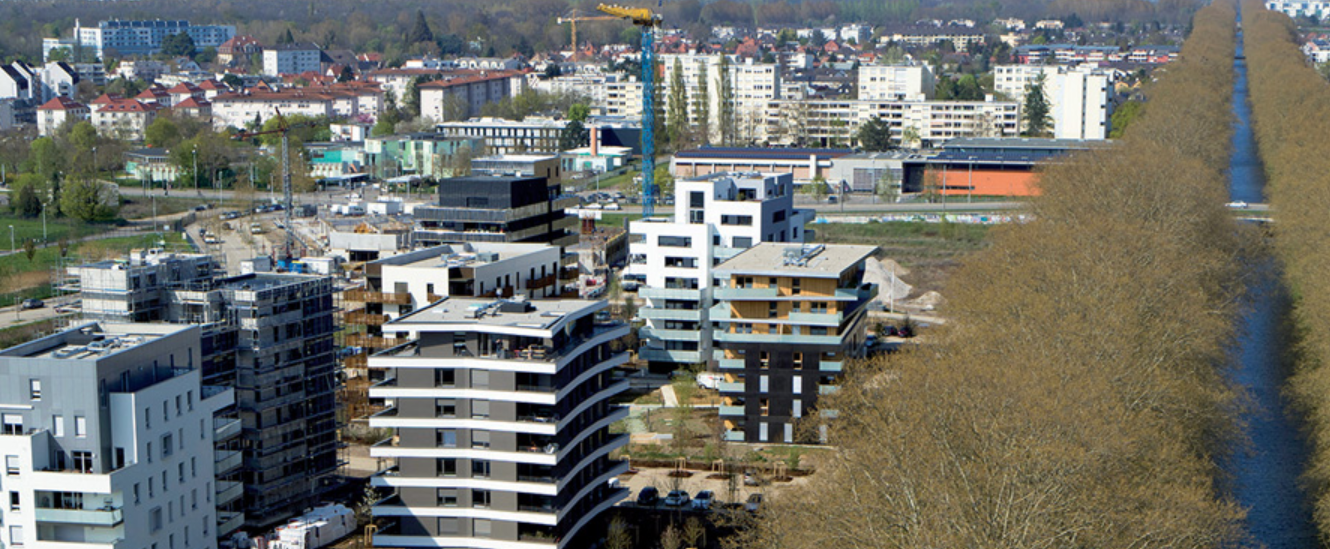
\includegraphics[width=15cm]{prairiescanal.png}
\end{center}
\caption{L'écoquartier Les Prairies du Canal en cours de construction}
\end{figure}







\chapter{Analyse de l'existant}

Intro

\section{Partie 1}

Intro

\subsection{Sous-partie 1}

Bla

\subsection{Sous-partie 2}

Bla\\

Transition

\section{Partie 2}

Bla\\

Transition

\section{Bilan récapitulatif}

Voici un tableau (cf. fig. 2.1) récapitulatif de notre analyse de l'existant...\\

%tableau centré à taille variable qui s'ajuste automatiquement suivant la longueur du contenu
\begin{figure}[!h]
\begin{center}
\begin{tabular}{|l|l|l|l|l|}
  \hline
  Solution & Critère 1 & Critère 2 & Critère 3 & Critère 4\\
  \hline
  Solution 1(cf. ref. \cite{cite0}) & Oui & Oui & Oui & Oui \\
  Solution 2(cf. ref. \cite{cite1}) & Oui & Oui & Oui & Non \\
  Solution 3(cf. ref. \cite{cite2}) & Oui (sauf telle chose) & Non & Non & Oui\\
  Solution 4(cf. ref. \cite{cite3}) & Oui& Non & Oui & Non\\
  Solution 5(cf. ref. \cite{cite4}) & Oui (uniquement ceux-ci) & Non & Oui & Non\\
  \hline
\end{tabular}
\end{center}
\caption{Tableau récapitulatif des solutions}
\end{figure}

 
\chapter{Analyse des besoins}

\chapter{Autre partie}

Dans cette partie nous cherchons à décrire dans un premier temps [...], puis, c[...].

\section{Partie 1}

Intro

\subsection{Sous-partie 1}

\begin{figure}[!ht]
\begin{center}

\includegraphics[height=12cm]{autre_partie/image1}
\end{center}
\caption[autre partie générale]{autre partie image 1\protect\footnotemark}
%\floatfoot{Source: (Citation command)}
% avec le package "floatrow"
\end{figure}

%footnote protected pour apparaitre dans la légende d'une image
\footnotetext{Schéma d'après : \textit{Auteur 1 \& Propriétaire image}, LICENCE (cf. ref. \cite{cite4})}

\newpage{}

\subsection{Sous-partie 2}

\begin{figure}[!ht]
\begin{center}

\includegraphics[height=12cm]{autre_partie/image2}
\end{center}
\caption[autre partie]{autre partie globale de notre quelque chose}
\end{figure}

Nous retrouvons ici, blabla\footnote{Application bla - Interface blabla} [...].

\subsubsection{Sous-sous-partie 1}

Le bla (cf. ref. \cite{cite6}) est [...]:

\begin{itemize}
\item item1;
\item item2;
\item item3;
\item item4;
\item item5.
\end{itemize}

\newpage

\subsubsection{Sous-sous-partie 2}

%Les lignes :
% \setcounter{secnumdepth}{4}
% \setcounter{tocdepth}{4}
%dans le fichier "main.tex" permettent de faire en sorte que les paragraphes soient interprété comme des titres de niveau 5
\paragraph{Paragraphe 1 (agissant comme titre niveau 5)}
%forcer un saut de ligne
~\\
\hskip7mm

\begin{figure}[!ht]
\begin{center}

\includegraphics[height=6cm]{autre_partie/image3}
\end{center}
\caption[Structure d'unz autre chose]{Structure d'une autre chose\protect\footnotemark}
\end{figure}

Ce schéma représente bla.

\footnotetext{Schéma et explication d'après le wiki bla (cf. ref. \cite{cite0})}

\paragraph{Paragraphe 2}
~\\
\hskip7mm

%fixer les floats précédemment définis
%\FloatBarrier

Bla

\subparagraph{Sous-paragraphe 1}
~\\
\hskip7mm

Bla

\begin{figure}[H]
\begin{center}

\includegraphics[height=10cm]{autre_partie/image4}
\end{center}
\caption{Diagramme de truc}
\end{figure}

\subparagraph{Sous-paragraphe 2}
~\\
\hskip7mm

Bla\\

Bla

\subparagraph{Sous-paragraphe 3}
~\\
\hskip7mm

Bla

\subsubsection{Sous-sous-partie 3}

Bla

\section{Partie 2}

Bla

\footnotetext{D'après le schéma disponible sur la documentfation officielle disponible sur le site blalbla}

Bla

\subsection{Sous-partie 1}

Bla

\subsection{Sous-partie 2}

Bla

\paragraph*{Paragraphe 1 (n'apparaitra pas dans l'index)}
Bla

\paragraph*{Paragraphe 2}
Bla

\paragraph*{Paragraphe 3}
Bla

\subsection{Sous-partie 3}

Bla

\chapter{Résultats}

\section{Partie 1}

Intro

\subsection{Sous-partie 1}

\paragraph*{Paragraphe 1 (n'apparaitra pas dans l'index)} Bla

\paragraph*{Paragraphe 2} Bla

\paragraph*{Paragraphe 3} Bla

\subsection{Sous-partie 2}

Bla

\subsection{Sous-partie 3}

Bla

\section{Partie 2}

Intro

\subsection*{Sous-partie 1 ('apparaitra pas dans l'index)} Bla

\paragraph*{Paragraphe 1 ('apparaitra pas dans l'index)} Bla

\paragraph*{Paragraphe 2} Bla

\paragraph*{Paragraphe 3} Bla

\newpage

\subsection*{Sous-partie 2}

Bla

%galerie d'image
\begin{figure}[htp]
  \centering
  \subfloat[Première image]{\label{fig:première}
\includegraphics[scale=0.8]{resultats/gallerie}}
  ~ %espace entre deux images sur une même ligne
  \subfloat[Deuxième image]{\label{fig:deuxième}
\includegraphics[scale=0.8]{resultats/gallerie}}
  ~
  \subfloat[Troisième image]{\label{fig:troisième}
\includegraphics[scale=0.8]{resultats/gallerie}}
  ~\\ %saute une ligne dans la galerie d'image
  \subfloat[Quatrième image]{\label{fig:quatrième}
\includegraphics[scale=0.8]{resultats/gallerie}}
  ~
  \subfloat[Cinquième image]{\label{fig:cinquième}
\includegraphics[scale=0.8]{resultats/gallerie}}
  \caption{Différents screenshots quelque chose, en gallerie}
  \label{fig:gallerie1}
\end{figure}

\chapter{Bilan}

%Rappel du context
Intro / Rappel Contexte

Nous avons donc pu en tirer la problématique suivante :

\begin{center}
\hskip7mm
Problématique du sujet
\end{center}

Bla

Bla\\

Bla\\

%Rappel des résultats
Bla

Bla\\

Bla

Bla

\newpage

%Conclusion/Perspectives
Bla

Bla\\

Bla

%Ne pas numéroter cette partie
\part*{Annexes}
%Rajouter la ligne "Annexes" dans le sommaire
\addcontentsline{toc}{part}{Annexes}

\chapter*{Annexe 1}
\addcontentsline{toc}{chapter}{Annexe 1}

%changer le format des sections, subsections pour apparaittre sans le num de chapitre
\makeatletter
\renewcommand{\thesection}{\@arabic\c@section}
\makeatother

%recommencer la numérotation des section à "1"
\setcounter{section}{0}

Intro

\section{Partie 1}

Bla

\subsection{Sous-partie 1}

Bla

\subsection{Sous-partie 2}

Bla

\subsection{Sous-partie 3}

Bla

\section{Partie 2}

Bla

\subsection{Sous-partie 1}

Bla

\subsection{Sous-partie 2}

Bla

\subsection{Sous-partie 3}

Bla

\chapter*{Annexe 2}
\addcontentsline{toc}{chapter}{Annexe 2}

%recommencer la numérotation des section à "1"
\setcounter{section}{0}

Intro

\section*{Prérequis}
\addcontentsline{toc}{section}{Prérequis}

Bla

\begin{itemize}
\item item1;
\item item2;
\item item3;
\item item4.
\end{itemize}

Bla

\section{Partie 1}

Bla

\subsection{Sous-parie 1}

Bla

\subsection{Sous-parie 2}

Bla

\section{Partie 2}

\begin{center}
\textsc{Attention !}

\textit{Texte d'avertissement}
\end{center}

Bla

\newpage

\section{Partie 3}

Bla

\begin{figure}[!ht]
\begin{center}
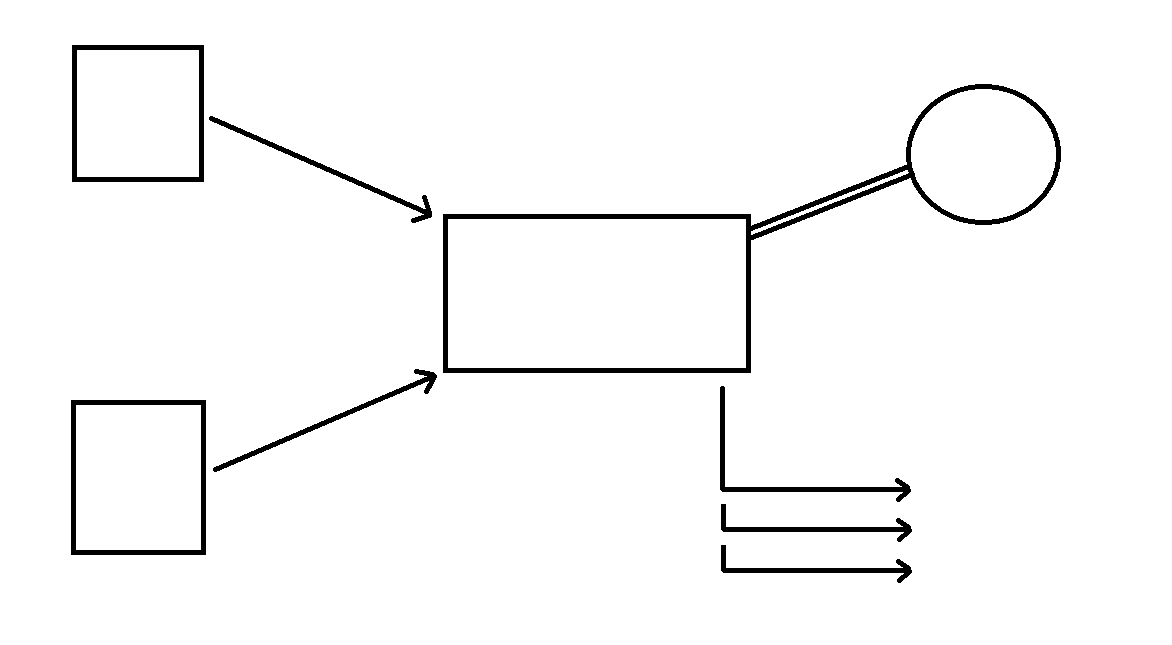
\includegraphics[height=8cm]{presentation/schema}
\end{center}
\caption[schema]{Presentation schema}
\end{figure}

\paragraph*{Paragraphe 1}
~\\
\hskip7mm

Bla

\paragraph*{Paragraphe 2}
~\\
\hskip7mm

Bla

\paragraph*{Paragraphe 3}
~\\
\hskip7mm

Bla

\newpage

%récupérer les citation avec "/footnotemark"
\nocite{*}

%choix du style de la biblio
\bibliographystyle{plain}
%inclusion de la biblio
\bibliography{bibliographie.bib}
%voir wiki pour plus d'information sur la syntaxe des entrées d'une bibliographie

\end{document}